\begin{frame}{The Japanese Conscription system}
    \begin{itemize}
        \item Japan required all 20-year-old males to participate in the military.

        \item The primary test assigned applicants to titles based on health.
        
        \begin{enumerate}
            \item Active Service: Sent to battlefield for 2-3 years.
            \item Replacement Service.
            \item Exemption.
        \end{enumerate}

        \item Militants return as reservists after 2-3 years of service.

        \item Reservists were called back into the battlefields in wartime. 
    \end{itemize}
\end{frame}

\begin{frame}
\begin{figure}
    \centering
    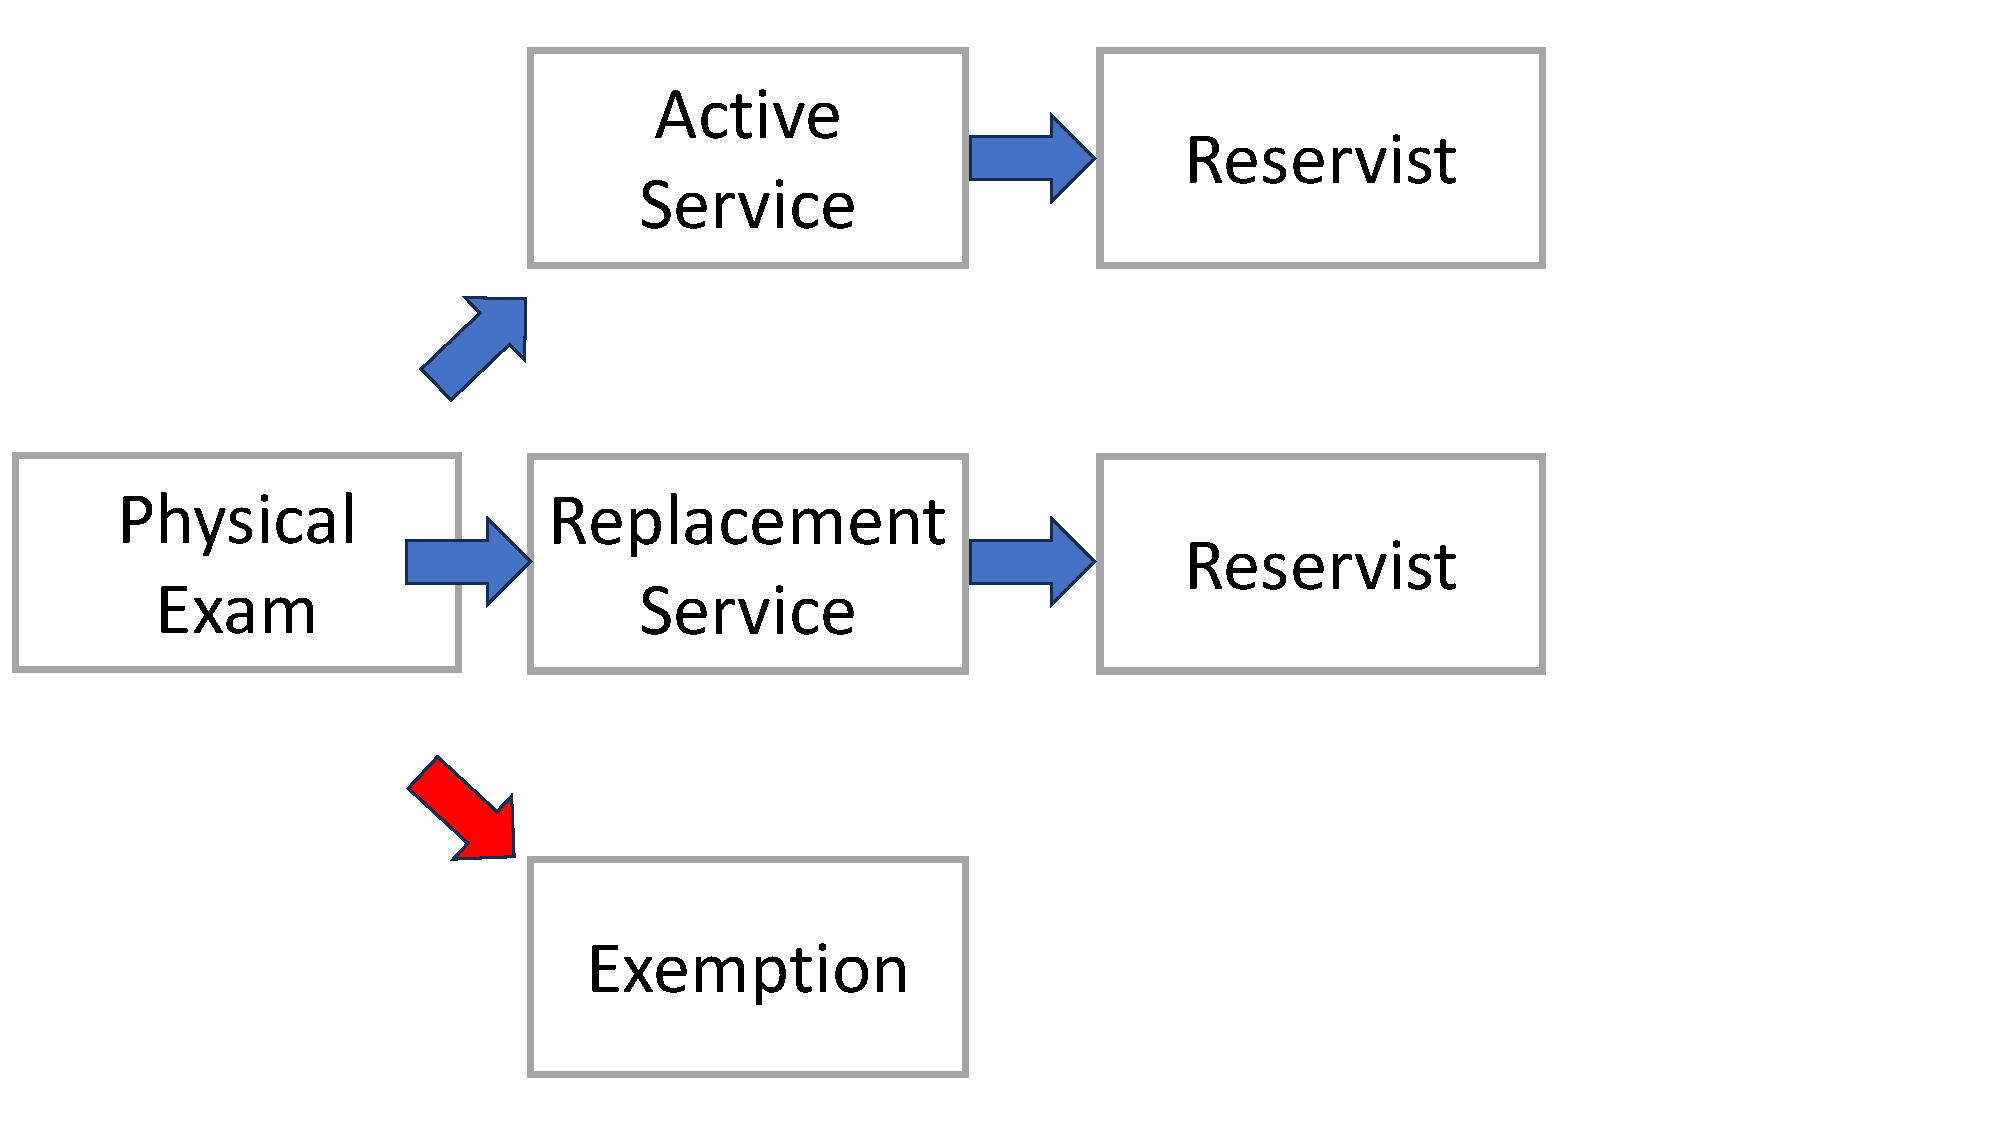
\includegraphics[width=1.3\linewidth]{Background/Drafting.pdf}
    \caption{Drafting Process}
    \label{fig:drafting}
\end{figure}
\end{frame}

\begin{frame}
\begin{figure}
    \centering
    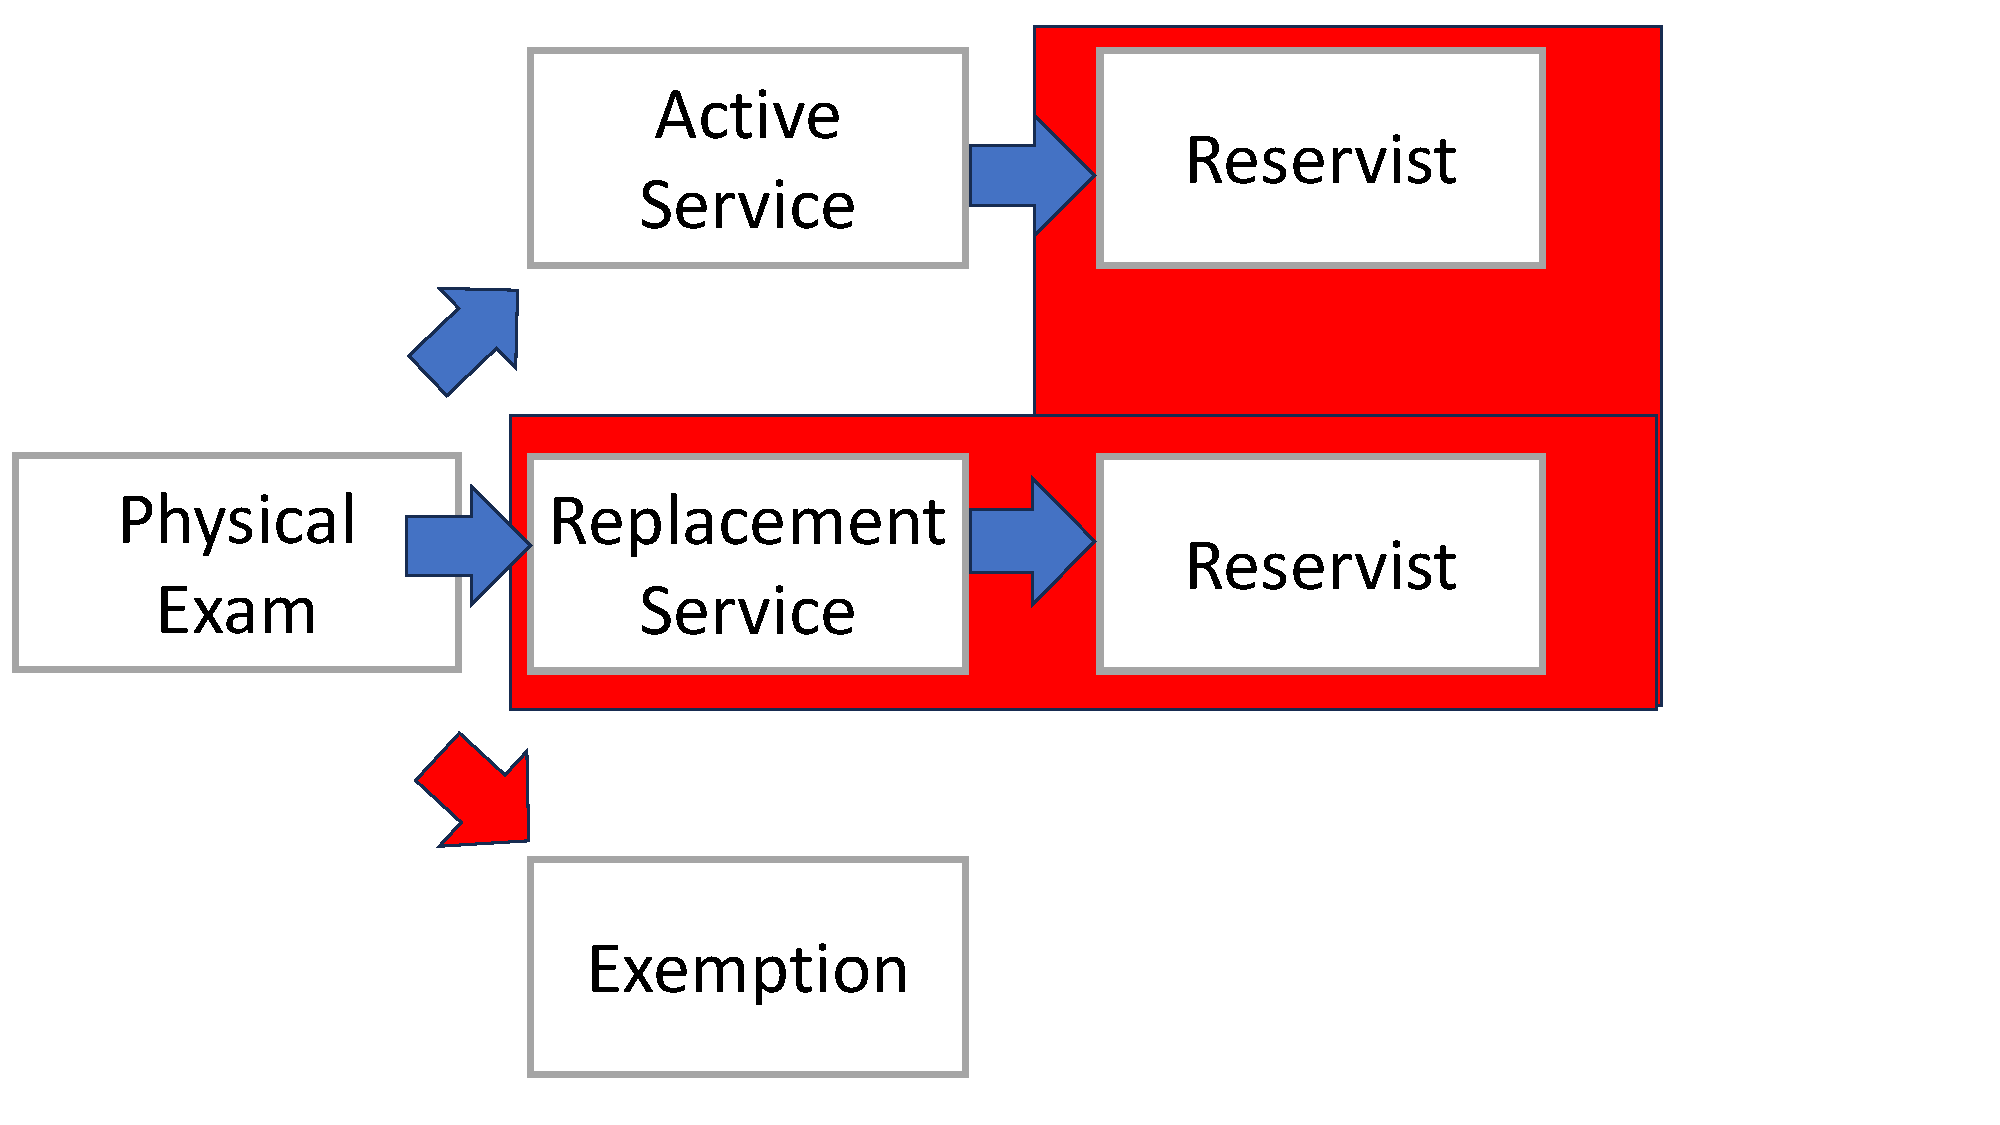
\includegraphics[width=1.3\linewidth]{Background/DraftRule-2.pdf}
    \caption{Draft Rules}
    \label{fig:draft-rule}
\end{figure}
\end{frame}